% \documentclass{beamer}
% \documentclass[aspectratio=169]{beamer}
\documentclass[aspectratio=169]{beamer}
\usetheme{boxes}
\usecolortheme{default}
% To get numbers in reference list
\setbeamertemplate{bibliography item}{\insertbiblabel}

\usepackage[utf8]{inputenc}
\usepackage[english]{babel}
\usepackage{graphicx,wrapfig,lipsum}

% \let\theorem\relax
\usepackage{amsmath,amsthm}
\newtheorem{theorem}{Theorem}

% \graphicspath{{images/}{images/logos/}{./}{../poster/images/}{../figures/}}

\title{Detecting Echo Chambers in social media; a graph-based approach}

\author[Francesco Zappia]{Francesco Zappia\inst{1} \\\footnotesize{Stefan
		Neumann\inst{1} \and Aris Anagnostopoulos\inst{2} \\ Aris Gionis\inst{1} }}
\institute{\inst{1} {\small  KTH Royal Institute of Technology} \and %
	\inst{2} {\small Sapienza University of Rome}}

% \author[Francesco Zappia]{Francesco Zappia}
% \institute{}

% \institute[] % (optional, but mostly needed)
% {\normalsize  KTH Royal Institute of Technology}
% - Use the \inst command only if there are several affiliations.
% - Keep it simple, no one is interested in your street address.

\date[\today] % (optional, should be abbreviation of conference name)
{\small\today}

% - Either use conference name or its abbreviation.
% - Not really informative to the audience, more for people (including
%   yourself) who are reading the slides online

% \subject{Theoretical Computer Science}
% This is only inserted into the PDF information catalog. Can be left
% out. 


% If you have a file called "university-logo-filename.xxx", where xxx
% is a graphic format that can be processed by latex or pdflatex,
% resp., then you can add a logo as follows:

% \pgfdeclareimage[height=0.5cm]{university-logo}{university-logo-filename}
% \logo{\pgfuseimage{university-logo}}


% Delete this, if you do not want the table of contents to pop up at
% the beginning of each subsection:


% If you wish to uncover everything in a step-wise fashion, uncomment
% the following command: 

%\beamerdefaultoverlayspecification{<+->}

% \setbeamerfont{caption}{size=\footnotesize}
% \usepackage[justification=centering]{caption}

\setbeamertemplate{background canvas}{%
	
\includegraphics[width=\paperwidth,height=\paperheight]{KTH-canvas}
}


\usepackage{caption}
\usepackage{subcaption}

\logo{
	% \includegraphics[height=0.6cm]{ERC_Rebound_Logo-1}%
	% \hspace{0.1cm}%
	% \includegraphics[height=0.7cm]{ERC_LOGO}%
	% \hspace{0.1cm}%
}


\begin{document}

\begin{frame}
	\titlepage
\end{frame}

\begin{frame}[c]
	\frametitle{Social media and Echo Chambers}
	\begin{itemize}
		\item Social media are more and more diffused
		\item On these platforms we experience every day phenomenons like
		      polarization and \textbf{Echo Chambers}
		\item Echo chambers correspond to groups of users with the same ideas
		      who, after interacting, reinforce their initial opinions
	\end{itemize}
	\begin{figure}
		\centering
		\includegraphics[width=0.3\linewidth]{../../tex/img/sample-graph.png}
	\end{figure}

\end{frame}

\begin{frame}[c]
	\frametitle{Data model: Contents and Threads}
	Our definition of Echo Chamber is based on the concepts of
	\textbf{Contents} and \textbf{Threads}

	\begin{itemize}
		\item \textbf{Content}: the resource which is discussed. We can
		      generally think of it as an online newspaper article. It is
		      identified by a URL, e.g.
		      \begin{center}
			      \url{https://www.breitbart.com/politics/2020/12/18/report-mark-zuckerbergs-.../}
		      \end{center}
		      \pause
		\item \textbf{Thread}: the social media \emph{locality} discussing a
		      content. Identified by its URL, e.g.
		      \begin{center}
			      \url{https://twitter.com/DineshDSouza/status/1340726209446113280}
		      \end{center}
	\end{itemize}
\end{frame}

\begin{frame}[c]
	\frametitle{Content and threads: an example}
	\begin{figure}
		\centering
		
\includegraphics[width=0.8\linewidth]{img/contents.png}
	\end{figure}
\end{frame}

\begin{frame}[c]
	\frametitle{Data model: Echo Chambers (1)}
	\begin{itemize}
		\item We focus on \textbf{controversial contents}, i.e.\ contents that
		      trigger a lot of hostile interactions \emph{globally}. Common
		      examples of controversial contents are politics and football
		      \pause
		\item We look for all the \textbf{threads associated to the content},
		      i.e.\ all discussions referencing the content URL
	\end{itemize}
	\bigskip
	\pause

	We can now give an initial informal definition of Echo Chambers.
	\begin{itemize}
		\item \textbf{Echo Chambers}: users discussing controversial contents
		      with mostly friendly interactions
	\end{itemize}
\end{frame}

\begin{frame}[c]
	\frametitle{Some graph concepts}
	Before formalizing this idea, we need to introduce two concepts

	\begin{itemize}
		\item \textbf{Signed graphs}: graph with positive and negative edges
		      \pause
		\item \textbf{Multiplex graph}: graph with multiple layers. Each layer
		      has the same set of vertices but its own set of edges
	\end{itemize}

	\begin{figure}
		\centering
		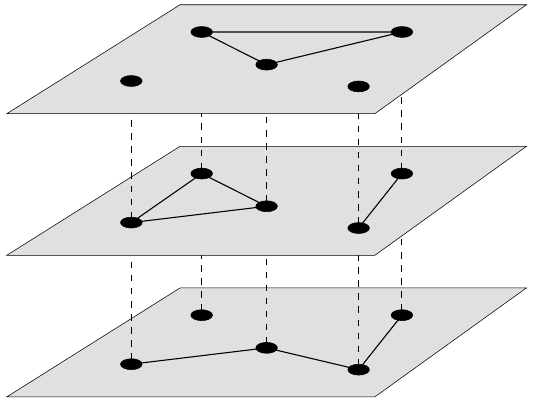
\includegraphics[width=0.3\linewidth]{../../tex/img/multiplex-graph.png}
	\end{figure}

\end{frame}

\begin{frame}[c]
	\frametitle{Data model: the interaction graph (1)}
	\begin{itemize}
		\item We construct the \textbf{interaction graph}: a weighted signed
		      multiplex graph
		      \begin{itemize}
			      \item Vertices represent users
			            \pause
			      \item Edges represent interactions between users
			            \pause
			      \item Edge weights $w_e \in [-1, 1]$
			            \pause
			      \item {\color{red}Negative} edge: hostile interaction.
				            {\color{green}Positive} edge: friendly interaction
			            \pause
			      \item Each layer is associated to a thread
		      \end{itemize}
	\end{itemize}
	\pause
	\begin{figure}
		\centering
		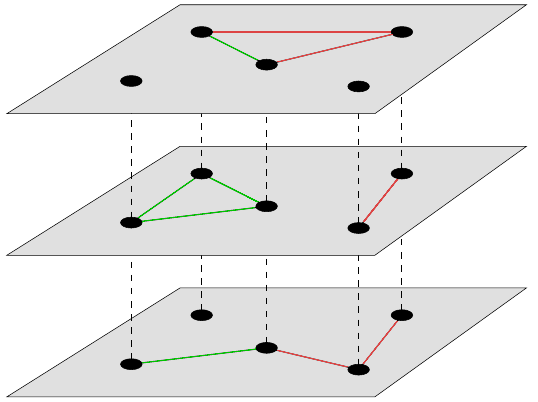
\includegraphics[width=0.3\linewidth]{img/multiplex-signed-graph.png}
	\end{figure}
\end{frame}

% \begin{frame}[c]
%     \frametitle{Data model: controversial contents and threads}
%     We define $\eta(T)$ to be the ratio between the number of
%     negative edges and the total number of edges in the layer associated to thread
%     $T$.
%     \pause
%     \begin{definition}[Controversial thread]
%         Let $\alpha \in [0,1]$. A thread (or content) is \emph{controversial} if
%         $\eta(T) > \alpha$ (or, similarly, $\eta(C) > \alpha $). Conversely, a
%         thread (or content) is \emph{non-controversial} if $\eta(T) \leq \alpha$
%         ($\eta(C) \leq \alpha$).
%     \end{definition}
% \end{frame}


\begin{frame}[c]
	\frametitle{Data model: Echo Chambers (2)}

	\begin{itemize}
		\item \textbf{Echo Chambers}: users discussing controversial contents
		      with mostly friendly interactions
		      \pause
		      \medskip
		      \begin{center}
			      \bigg\downarrow
		      \end{center}
		      \medskip
		\item Consider only \emph{non-controversial} threads associated to
		      \emph{controversial} contents
		      \begin{itemize}
			      \item \emph{Controversial}: more than $\alpha $ percent of
			            edges is negative
		      \end{itemize}
	\end{itemize}


\end{frame}

\begin{frame}[c]
	\frametitle{Data model: $\mathcal{S}_C$}
	\begin{itemize}
		\item $\mathcal{S}_C (U)$ contains threads which are \emph{locally}
		      non-controversial but it is defined only for contents that are
		      \emph{globally} controversial.
	\end{itemize}
	\begin{figure}
		\centering
		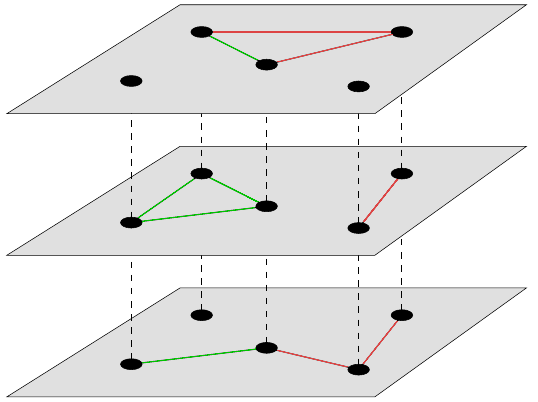
\includegraphics[width=0.3\linewidth]{img/multiplex-signed-graph.png}
	\end{figure}
\end{frame}

\begin{frame}[c]
	\frametitle{Data model: Echo Chambers (3)}

	\begin{itemize}
		\item \textbf{Echo Chambers}: users discussing controversial contents
		      with mostly friendly interactions
		      \medskip
		      \begin{center}
			      \bigg\downarrow
		      \end{center}
		      \medskip
		\item Consider only \emph{non-controversial} threads associated to
		      \emph{controversial} contents
		      \begin{equation*}
			      \xi(U) = \sum^{}_{C \in \hat{\mathcal{C}} } \sum^{}_{T[U] \in S_C (U)}
			      (| T^{+} [U] | - | T^{-} [U] |)
		      \end{equation*}
		      \begin{itemize}
			      \item $T[U]$ is the subgraph induced by $U$ in $T$
			      \item $|T^{+}[U]|$ is the number of positive edges in $T[U]$
		      \end{itemize}
		      \textbf{Echo Chamber Problem}: find vertices $U$ maximizing
		      $\xi(U)$.
	\end{itemize}


\end{frame}

\begin{frame}[c]
	\frametitle{The Echo Chamber Problem: our results (1)}
	\begin{itemize}
		\item We propose new methods for detecting echo
		      chambers in social media: the Echo Chamber Problem
		      \pause
		\item We show that it is hard to approximate this problem
		      \pause
		\item We propose MIP and heuristic for solving it
		      \pause
		\item The heuristic achieves good performances on synthetic data
		      \pause
		\item It has limitations on real-world data
	\end{itemize}
	\pause
	We will not show the proofs for our results.
\end{frame}

\begin{frame}[c]
	\frametitle{The Echo Chamber Problem: our results (2)}
	% We need to introduce a concept first.
	%
	% \pause
	% \bigskip
	%
	% Algorithm $A$ is an $r$-approximation algorithm for a given maximization
	% problem if it always finds a solution which is at most $1/r$ times the
	% optimal in polynomial time.
	%
	% \pause
	% \bigskip

	The Echo Chamber Problem cannot be approximated in polynomial time for a non-trivial factor.
	\begin{theorem}
		The \acrfull{ECP} has no $n^{1-\epsilon} $-approximation algorithm for
		any $\epsilon > 0$ unless $\mathcal{P} = \mathcal{NP}  $.
	\end{theorem}

\end{frame}

\begin{frame}[c]
	\frametitle{The Echo Chamber Problem: our results (3)}
	An exact solution for the problem can be found through the following Mixed
	Integer Programming (MIP) Model

		{\footnotesize
			\begin{alignat}{3}
				\label{eq:ecp-exact1}
				\text{maximize}     &                                                 & \sum_{ T_{k} \in \mathcal{T}_{C}, \; C \in
					\mathcal{\hat{C}} } \big( \sum^{}_{ij \in E^{+}_k } x_{ij}
				^{k} - \sum_{ij \in E^{-}_k } x_{ij} ^{k} \big)                                                                                                                                               \\
				\label{eq:ecp-v1}
				\text{subject to}   & \quad                                           & x _{ij}^{k}  \leq y_i                                               & \quad \forall ij \in E_k                        \\
				\label{eq:ecp-v2}
				                    &                                                 & x _{ij}^{k}  \leq y_j                                               & \quad \forall ij \in E_k                        \\
				\label{eq:ecp-t1}
				                    &                                                 & x _{ij}^{k}  \leq z_k                                               & \quad \forall ij \in E_k                        \\
				\label{eq:ecp-e1}
				                    &                                                 & x _{ij} ^{k} \geq - 2 + y_i + y_j + z_k                             & \quad \forall ij \in E_k                        \\
				\label{eq:ecp-alpha-constraint1}
				                    &                                                 & \sum^{}_{ij \in E_k^{-} } x_{ij}^{k}  - \alpha \sum^{}_{ij \in E_k}
				x_{ij} ^{k}  \leq 0 & \quad \forall T_{k} \in \mathcal{T} _{C}, C \in
				\hat{\mathcal{C}}                                                                                                                                                                             \\
				\label{eq:ecp-vertex-def1}
				                    &                                                 & y _{i} \in  \{0, 1\}                                                & \quad \forall i \in V                           \\
				\label{eq:ecp-edge-def1}
				                    &                                                 & 0 \leq x _{ij} ^{k}  \leq 1                                         & \quad \forall ij \in E_k                        \\
				\label{eq:ecp-thread-def1}
				                    &                                                 & 0 \leq z _{k} \leq 1                                                & \quad \forall T_{k} \in \mathcal{T} _{C}, C \in
				\hat{\mathcal{C}}
			\end{alignat}
		}

\end{frame}

\begin{frame}[c]
	\frametitle{An heuristic for the Echo Chamber Problem}
	We propose a heuristic for solving the Echo Chamber Problem

	\begin{itemize}
		\item It is based on the relaxation of the MIP (integrality constraints
		      are removed)
		\item Each edges is assigned a value in the MIP. This heuristic
		      considers the vertices associated to edges with the highest value
		      as possible solutions
	\end{itemize}
\end{frame}

\begin{frame}[c]
	\frametitle{Echo Chamber Problem Validation}
	\begin{itemize}
		\item No benchmark is available for such a problem
		      \pause
		\item We use the Echo Chamber problem to find users in the same
		      community
		      \pause
		      \begin{center}
			      $\downarrow$ \\
			      Clustering problem
		      \end{center}
	\end{itemize}
\end{frame}

% \begin{frame}[c]
%     \frametitle{Data Generation (1)}
%     We generate synthetic data to evaluate the algorithms.
%     \begin{itemize}
%         \item A group of communities with positive edges between vertices
%               inside the same community and negative edges between vertices in
%               different communities
%         \item We flip a fraction of edges represented by $x$ and measure how
%               good the clustering is
%     \end{itemize}
% \end{frame}
%
% \begin{frame}[c]
%     \frametitle{Data Generation (1)}
%     \begin{figure}[htpb]
%         \centering
%         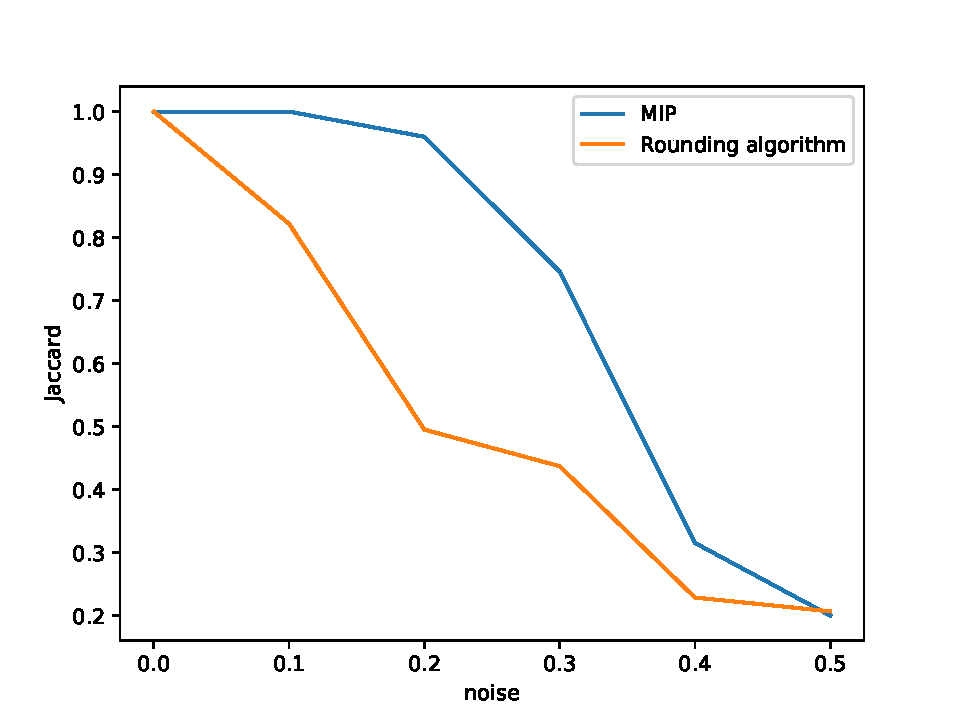
\includegraphics[width=0.8\linewidth]{../../tex/out/synthetic/noise_jaccard.pdf}
%         \caption{Jaccard scores obtained by the Exact MIP and rounding
%             algorithm}%
%         \label{fig:jaccard}
%     \end{figure}
%
% \end{frame}

\begin{frame}[c]
	\frametitle{Data collection}
	\begin{itemize}
		\item Graphs are built from Reddit or Twitter
		      \visible<1->{
		\item Similar data collection process:
		      \begin{itemize}
			      \item Retrieve contents from posts of a \emph{subreddit} or
			            of a Twitter account
			      \item Retrieve all threads related to that contents
		      \end{itemize}}
		      \visible<3->{
		\item Edge labels are obtained through a \emph{sentiment analyzer}}
	\end{itemize}

	\visible<2->{
		\begin{figure}[htpb]
			\centering
			
\includegraphics[width=0.4\linewidth]{img/twitter.png}
		\end{figure}}
\end{frame}

\begin{frame}[c]
	\frametitle{Data collection and generation}
	We obtained labeled datasets with different techniques
	\pause
	\begin{itemize}
		\item We generate synthetic data
		      \pause
		\item r/asktrumpsupporters asks users to choose a flair among
		      \emph{Trump Supporter}, \emph{Non Supporter} and \emph{Undecided}
		      \pause
		\item Twitter users are labeled according to the politicians they
		      follow (if they are mostly \emph{democrat} or \emph{republican}).
		      This dataset is built on @nytimes.
	\end{itemize}

	\begin{figure}
		\centering
		
\includegraphics[width=0.4\linewidth]{img/flairs.png}
	\end{figure}
\end{frame}

\begin{frame}[c]
	\frametitle{Rounding algorithm evaluation}
	Observations on the results
	\begin{itemize}
		\visible<1->{
		\item The rounding algorithm is able to reconstruct communities in synthetic data
		      }
		      \visible<2->{
			      \begin{figure}
				      \centering
				      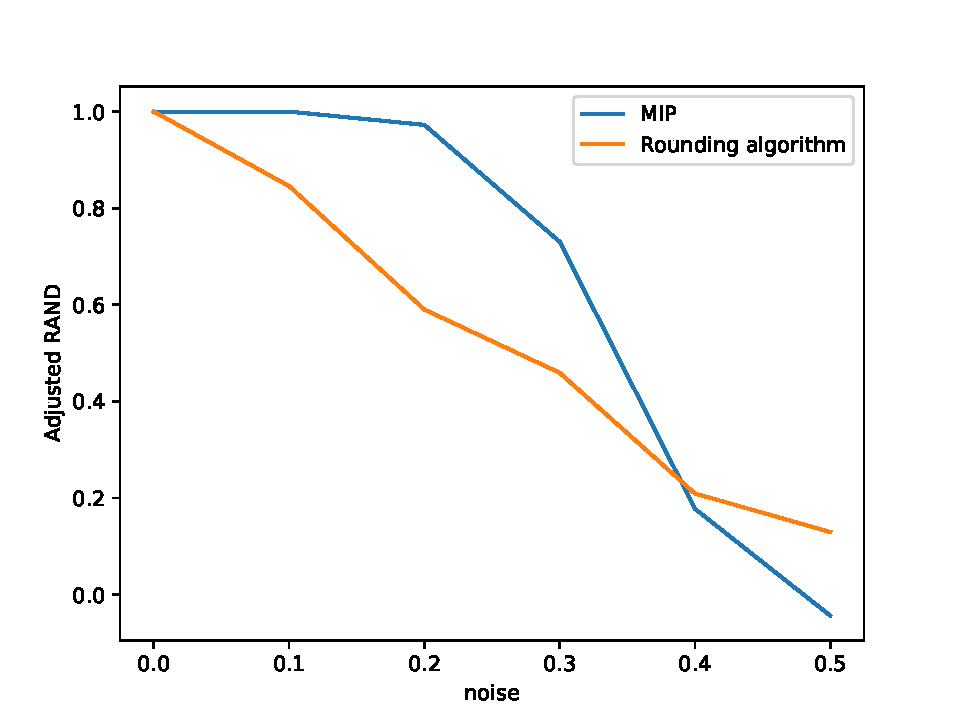
\includegraphics[width=0.3\linewidth]{../../tex/out/synthetic/noise_adj_rand.pdf}
			      \end{figure}
		      }
		      \visible<3->{
		\item It has limitations on real-world data (Adjusted RAND $< 0.1$)}
		      \visible<4->{
		\item Different reasons}
		      \begin{itemize}
			      \visible<5->{
			      \item Non-validity of data model}
			            \visible<6->{
			      \item Complexity of internet communication and sentiment
			            analyzer}
			            \visible<7->{
			      \item Limitations of the rounding algorithm}
			            \visible<8->{
			      \item Sparsity of the data}
		      \end{itemize}
	\end{itemize}
\end{frame}



\begin{frame}[c]
	\frametitle{Conclusions}
	Our idea is that we may not be evaluating properly our heuristic
	\begin{itemize}
		\item The experiments on synthetic data show good
		      performances
		\item Limitations are observed only on real-world data
		      \pause
		\item Need for a more accurate validation method
	\end{itemize}

	\pause
	\bigskip

	Also, we propose new and alternative formulations
	\begin{itemize}
		\pause
		\item Density can be taken into account
		      \pause
		\item Formulation can be extended with \emph{follow graph}
	\end{itemize}

\end{frame}

\iffalse
	\begin{frame}[allowframebreaks]
		\frametitle{References}
		\bibliographystyle{apalike}
		\bibliography{citations}
	\end{frame}
\fi

\end{document}
